% Options for packages loaded elsewhere
\PassOptionsToPackage{unicode}{hyperref}
\PassOptionsToPackage{hyphens}{url}
%
\documentclass[
]{article}
\usepackage{amsmath,amssymb}
\usepackage{iftex}
\ifPDFTeX
  \usepackage[T1]{fontenc}
  \usepackage[utf8]{inputenc}
  \usepackage{textcomp} % provide euro and other symbols
\else % if luatex or xetex
  \usepackage{unicode-math} % this also loads fontspec
  \defaultfontfeatures{Scale=MatchLowercase}
  \defaultfontfeatures[\rmfamily]{Ligatures=TeX,Scale=1}
\fi
\usepackage{lmodern}
\ifPDFTeX\else
  % xetex/luatex font selection
\fi
% Use upquote if available, for straight quotes in verbatim environments
\IfFileExists{upquote.sty}{\usepackage{upquote}}{}
\IfFileExists{microtype.sty}{% use microtype if available
  \usepackage[]{microtype}
  \UseMicrotypeSet[protrusion]{basicmath} % disable protrusion for tt fonts
}{}
\makeatletter
\@ifundefined{KOMAClassName}{% if non-KOMA class
  \IfFileExists{parskip.sty}{%
    \usepackage{parskip}
  }{% else
    \setlength{\parindent}{0pt}
    \setlength{\parskip}{6pt plus 2pt minus 1pt}}
}{% if KOMA class
  \KOMAoptions{parskip=half}}
\makeatother
\usepackage{xcolor}
\usepackage[margin=1in]{geometry}
\usepackage{color}
\usepackage{fancyvrb}
\newcommand{\VerbBar}{|}
\newcommand{\VERB}{\Verb[commandchars=\\\{\}]}
\DefineVerbatimEnvironment{Highlighting}{Verbatim}{commandchars=\\\{\}}
% Add ',fontsize=\small' for more characters per line
\usepackage{framed}
\definecolor{shadecolor}{RGB}{248,248,248}
\newenvironment{Shaded}{\begin{snugshade}}{\end{snugshade}}
\newcommand{\AlertTok}[1]{\textcolor[rgb]{0.94,0.16,0.16}{#1}}
\newcommand{\AnnotationTok}[1]{\textcolor[rgb]{0.56,0.35,0.01}{\textbf{\textit{#1}}}}
\newcommand{\AttributeTok}[1]{\textcolor[rgb]{0.77,0.63,0.00}{#1}}
\newcommand{\BaseNTok}[1]{\textcolor[rgb]{0.00,0.00,0.81}{#1}}
\newcommand{\BuiltInTok}[1]{#1}
\newcommand{\CharTok}[1]{\textcolor[rgb]{0.31,0.60,0.02}{#1}}
\newcommand{\CommentTok}[1]{\textcolor[rgb]{0.56,0.35,0.01}{\textit{#1}}}
\newcommand{\CommentVarTok}[1]{\textcolor[rgb]{0.56,0.35,0.01}{\textbf{\textit{#1}}}}
\newcommand{\ConstantTok}[1]{\textcolor[rgb]{0.00,0.00,0.00}{#1}}
\newcommand{\ControlFlowTok}[1]{\textcolor[rgb]{0.13,0.29,0.53}{\textbf{#1}}}
\newcommand{\DataTypeTok}[1]{\textcolor[rgb]{0.13,0.29,0.53}{#1}}
\newcommand{\DecValTok}[1]{\textcolor[rgb]{0.00,0.00,0.81}{#1}}
\newcommand{\DocumentationTok}[1]{\textcolor[rgb]{0.56,0.35,0.01}{\textbf{\textit{#1}}}}
\newcommand{\ErrorTok}[1]{\textcolor[rgb]{0.64,0.00,0.00}{\textbf{#1}}}
\newcommand{\ExtensionTok}[1]{#1}
\newcommand{\FloatTok}[1]{\textcolor[rgb]{0.00,0.00,0.81}{#1}}
\newcommand{\FunctionTok}[1]{\textcolor[rgb]{0.00,0.00,0.00}{#1}}
\newcommand{\ImportTok}[1]{#1}
\newcommand{\InformationTok}[1]{\textcolor[rgb]{0.56,0.35,0.01}{\textbf{\textit{#1}}}}
\newcommand{\KeywordTok}[1]{\textcolor[rgb]{0.13,0.29,0.53}{\textbf{#1}}}
\newcommand{\NormalTok}[1]{#1}
\newcommand{\OperatorTok}[1]{\textcolor[rgb]{0.81,0.36,0.00}{\textbf{#1}}}
\newcommand{\OtherTok}[1]{\textcolor[rgb]{0.56,0.35,0.01}{#1}}
\newcommand{\PreprocessorTok}[1]{\textcolor[rgb]{0.56,0.35,0.01}{\textit{#1}}}
\newcommand{\RegionMarkerTok}[1]{#1}
\newcommand{\SpecialCharTok}[1]{\textcolor[rgb]{0.00,0.00,0.00}{#1}}
\newcommand{\SpecialStringTok}[1]{\textcolor[rgb]{0.31,0.60,0.02}{#1}}
\newcommand{\StringTok}[1]{\textcolor[rgb]{0.31,0.60,0.02}{#1}}
\newcommand{\VariableTok}[1]{\textcolor[rgb]{0.00,0.00,0.00}{#1}}
\newcommand{\VerbatimStringTok}[1]{\textcolor[rgb]{0.31,0.60,0.02}{#1}}
\newcommand{\WarningTok}[1]{\textcolor[rgb]{0.56,0.35,0.01}{\textbf{\textit{#1}}}}
\usepackage{longtable,booktabs,array}
\usepackage{calc} % for calculating minipage widths
% Correct order of tables after \paragraph or \subparagraph
\usepackage{etoolbox}
\makeatletter
\patchcmd\longtable{\par}{\if@noskipsec\mbox{}\fi\par}{}{}
\makeatother
% Allow footnotes in longtable head/foot
\IfFileExists{footnotehyper.sty}{\usepackage{footnotehyper}}{\usepackage{footnote}}
\makesavenoteenv{longtable}
\usepackage{graphicx}
\makeatletter
\def\maxwidth{\ifdim\Gin@nat@width>\linewidth\linewidth\else\Gin@nat@width\fi}
\def\maxheight{\ifdim\Gin@nat@height>\textheight\textheight\else\Gin@nat@height\fi}
\makeatother
% Scale images if necessary, so that they will not overflow the page
% margins by default, and it is still possible to overwrite the defaults
% using explicit options in \includegraphics[width, height, ...]{}
\setkeys{Gin}{width=\maxwidth,height=\maxheight,keepaspectratio}
% Set default figure placement to htbp
\makeatletter
\def\fps@figure{htbp}
\makeatother
\usepackage{soul}
\setlength{\emergencystretch}{3em} % prevent overfull lines
\providecommand{\tightlist}{%
  \setlength{\itemsep}{0pt}\setlength{\parskip}{0pt}}
\setcounter{secnumdepth}{-\maxdimen} % remove section numbering
\ifLuaTeX
  \usepackage{selnolig}  % disable illegal ligatures
\fi
\IfFileExists{bookmark.sty}{\usepackage{bookmark}}{\usepackage{hyperref}}
\IfFileExists{xurl.sty}{\usepackage{xurl}}{} % add URL line breaks if available
\urlstyle{same}
\hypersetup{
  pdftitle={An introduction to R markdown},
  pdfauthor={Chris B. Wall -- cbwall@hawaii.edu},
  hidelinks,
  pdfcreator={LaTeX via pandoc}}

\title{An introduction to R markdown}
\author{Chris B. Wall --
\href{mailto:cbwall@hawaii.edu}{\nolinkurl{cbwall@hawaii.edu}}}
\date{12/11/2024}

\begin{document}
\maketitle

{
\setcounter{tocdepth}{3}
\tableofcontents
}
\hypertarget{this-is-an-r-markdown}{%
\subsection{This is an R Markdown!}\label{this-is-an-r-markdown}}

\emph{Please see the video here on how to download repository and get
set up} \textbf{\url{https://www.youtube.com/watch?v=MIxZdjMa5eo}}

R markdown is great, and when I say great, \textbf{I mean REALLY great.}

When exporting your markdown you can\ldots{}\\
\emph{(1) embed figures}\\
\emph{(2) view tables}\\
\emph{(3) export models}\\
\emph{(4) archive your data pipeline}

You can write code and execute functions in a similar way to normal R
script files. However, there are a few distinct differences between R
scripts and R markdown scripts. Some of these differences relate to how
code is executed. Other differences can be seen in the added benefit of
integrating scripts with outputs and other embedded properties.

The benefit of using markdown with colleagues is they can actually see
the script, the figures, the path of model selection, even the
assumptions of ANOVA (QQ plots, etc) that normally are hidden behind the
curtain.\\
In short, \textbf{R markdown helps make your science repeatable,
accessible, and data analysis coherent!}

Here are some common commands and examples of what Markdown can do for
you. I recommend visiting the
\href{https://bookdown.org/yihui/rmarkdown/}{R Bookdown for a complete
and exhaustive guide} or the
\href{https://www.rstudio.com/wp-content/uploads/2015/02/rmarkdown-cheatsheet.pdf}{R
markdown cheat sheet}

If you want to test yourself, the
\href{https://www.markdowntutorial.com/}{R Markdown tutorial} is another
great guide.

For the advanced Markdown-ers, you can also write and code a manuscript
in markdown that can be exported to Word, with references embedded.
Markdown magic!
\href{https://danovando.github.io/publications-with-rmarkdown/presentations/pubs-with-rmarkdown}{R
markdown: Publsihing workflows and manuscript.}

\hypertarget{markdown-basics}{%
\subsection{Markdown basics}\label{markdown-basics}}

Before we get started, \textbf{let us discuss version control and
software carpentry}. It is increasingly important for you to back up and
secure your data. This is not only true for your final data but also the
versions of your data on the way to the ``ultimate'' data version. Think
of this as a software update. First, you need to have a version of the
software; this version may change as your team/PI/committee or others as
for changes to your code. You can then update your code to reflect new
needs, while also maintaining an archive or what the code WAS. This is
in effect: version control. It helps you back up your work and maintain
an archive of where you were and where you are.

Now, carpentry. Having a simple, clear directory of data folders is
critical for making your data structure navigable. This is general house
keeping for your directory. It will make your code, output, and products
flow and keep your directory clean and organized.

Is this all above your head? That's okay. See some open access resources
here to help you get started in R (notice the pages are all R-Markdown
html objects!) and on the path to coding.
\href{https://datacarpentry.org/R-ecology-lesson/index.html}{R data
carpentry course}.

\hypertarget{first-git-with-r-projects}{%
\subsubsection{First: Git with R
Projects}\label{first-git-with-r-projects}}

My first advise to you would be to set up a
\href{https://github.com/}{GitHub account}. \textbf{Having a GitHub (or
other online repo) allows you to have all your code, markdown, figures,
data, etc archived online for safety and version control}. You can make
these repositories private or collaborative. It is easy! There are a lot
of resources out there on why/how to use GitHub, and you'll see why it
is important as you advance your carpentry--you can
\href{http://happygitwithr.com/big-picture.html}{read about how painless
this is}.

Whether you choose to GIT with it, or stick with running from your
device, you should start by making an \emph{R project} in R-Studio. You
can read all about how to do this at
\href{http://happygitwithr.com/rstudio-git-github.html}{happygitwithR.com}.

In R Studio you can run a Project from your local directory or make one
with version control by clicking the option to make an R project with
version control will set you on the path to linking with GitHub (if you
go this route, see
\href{http://happygitwithr.com/rstudio-git-github.html}{happygitwithR.com}
first, as you must set up a github account, then make a repository, then
use the repository URL to link to your R project). There are a few more
steps to integrating R and github now, since github has moved to
two-factor authentication, but you can see the
\href{https://docs.github.com/en/authentication/securing-your-account-with-two-factor-authentication-2fa/accessing-github-using-two-factor-authentication}{how
to} and some
\href{https://stackoverflow.com/questions/66065099/how-to-update-github-authentification-token-on-rstudio-to-match-the-new-policy}{trouble
shooting} in the linked sites.

If you decide to instead without version control, then set up the
project wherever you wish on your computer. When you set your ``R
Project'' directory, R Studio will generate a folder that houses your R
Project. From here you can create your Rmd file and folder directory as
you wish. For best practices, I recommend setting up a directory for
each project (\emph{see directory for this project below}).

From here, every time you open want to work on this project in R studio,
click on the Project. This will allow you to load data in a simple way
that anyone can understand (i.e., upload file ``symbiont.csv'', from
folder ``data'')--and it is easy to share this structure with
collaborators.

Yet another reason to use R Projects: it will eliminate the pesky and
sometimes overly personal directories we all have on our desktop aka:
``\textasciitilde/Desktop/PhD/WTFproject/NeverGoingToGetPublished/data.csv''

\begin{figure}
\centering
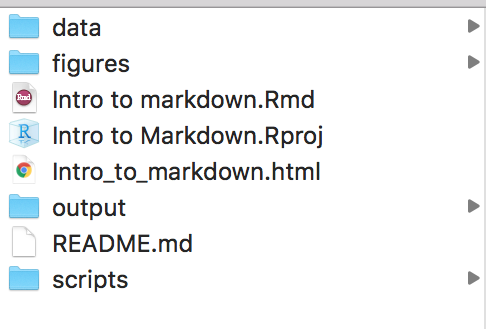
\includegraphics[width=0.3\textwidth,height=\textheight]{data/directory example.png}
\caption{\textbf{Figure 1. Data Directory example}}
\end{figure}

\hypertarget{common-commands}{%
\subsubsection{Common Commands}\label{common-commands}}

\emph{Notice the script at the very top of your markdown (this is not
standard, but is customized)}

\begin{center}\rule{0.5\linewidth}{0.5pt}\end{center}

output:\\
html\_document:\\
code\_folding: hide\\
toc: yes\\
toc\_depth: 3\\
toc\_float: yes ***

Let's go through this line by line\ldots{}

\begin{itemize}
\tightlist
\item
  \texttt{html\_document}: an option you originally set when you open
  the markdown. This is how your file will be exported.\\
\item
  \texttt{code\_folding:\ hide} will allow you to \emph{show} or
  \emph{hide} all code (option at top of file)\\
\item
  \texttt{toc}: for table of contents on the left\\
\item
  \texttt{toc\_depth}: how many header levels you will have in table of
  contents\\
\item
  \texttt{toc\_float}: lets your contents move as you advance in your
  document.
\end{itemize}

\emph{Play around with these options, and see how they affect your code}

There are other options too, such as \texttt{number\_sections:\ true} to
add numbering to your sections.

\hypertarget{the-setup-chunk}{%
\subsubsection{The setup chunk}\label{the-setup-chunk}}

\begin{itemize}
\item
  First, if you want to make a new chunk (where code is written), use
  the shortcut! \texttt{Control\ +\ Option\ +\ I"} will generate a new
  chunk for you
\item
  \texttt{r\ setup}: This is your set up code and is a useful way to get
  around the fact that knitr will look for your .Rmd file and all files
  in the this directory. By setting the root.dir you can force knitr to
  look for files in the directory you specify and the folders within.
\end{itemize}

In the setup chunk (the first code chunk) you can set `global' options,
such as message/warning exclusion, or hiding results or outputs.\\
\texttt{knitr::opts\_chunk\$set(warning=FALSE,\ message=FALSE)}: This
command here is requiring the package \texttt{knitr} in the code chunk
(`set' for set up) and is saying to ``make all warning and message
FALSE'' i.e., hide them from output.

\begin{itemize}
\item
  \texttt{include=FALSE}: this command makes your code absent from final
  html. It is executed but the code is hidden.
\item
  \texttt{eval=FALSE}: this command allows you to show the code in your
  script within R studio, but not evaluate (or run) the code. It is
  effectively silent in your analysis and output html.
\item
  \texttt{echo=FALSE}: this will show the output but not the code
  chunk\ldots{} notice the difference.
\item
  \texttt{results=\textquotesingle{}hide\textquotesingle{}}: this will
  hide all results in a code chunk, or any returned results from your
  commands.
\item
  \texttt{collapse\ =\ TRUE}: this is one of my new favorites. You enter
  this to your chunk options for a code chunk to run all the way through
  and not separate into pieces of results. This is usueful if you have
  lots of outputs (even if they are hidden using
  \texttt{results=\textquotesingle{}hide\textquotesingle{}}, the code
  chunk will still give breaks where results would be. Collapse = TRUE
  stops this.)
\end{itemize}

\hypertarget{text-formatting}{%
\subsubsection{Text formatting}\label{text-formatting}}

It is useful to understand how to modify text and format headings. You
can do this in a variety of ways.

\begin{itemize}
\item
  \texttt{line\ break}: this is executed by two spaces at the end of
  previous line, and a return
\item
  \texttt{headings}: use \texttt{\#} for headings, \texttt{\#}\ldots.
  \texttt{\#\#\#\#} and so on. \# is largest and \#\#\#\# smallest
  heading
\end{itemize}

\texttt{Italics} comes from two calls \emph{italics} or \emph{italics};
\texttt{bold} is done the same way \textbf{bold} and \textbf{bold}

\begin{itemize}
\item
  \texttt{Superscript} superscript\textsuperscript{2} or
  \texttt{strikethroughs} \st{strikethrough} can also be useful text
  modifiers.
\item
  \texttt{Subscript} subscript\textsubscript{2} are another useful one
  for chemistry CO\textsubscript{2},
  NO\textsubscript{3}\textsuperscript{-}, and the like\ldots{}
\item
  \texttt{add\ links} to urls like this \href{www.rstudio.com}{R studio
  link}
\item
  \texttt{endash} : --\\
\item
  \texttt{emdash}: ---\\
\item
  \texttt{ellipsis}: \ldots{}
\item
  \texttt{inline\ equation}: \(A = \pi*r^{2}\) or \(y = a*x+ b\)
\item
  (a line can inserted with \texttt{***})
\item
  using the \texttt{\textgreater{}} before and after a line can give you
  a quote/emphasis, such as\ldots{}
\end{itemize}

\begin{quote}
``Its Van Halen, not Van Hagar!''\\
- Garth Algar
\end{quote}

\begin{center}\rule{0.5\linewidth}{0.5pt}\end{center}

\hypertarget{code-chunks}{%
\subsubsection{Code chunks}\label{code-chunks}}

Code chunks are where your code is executed. If you do not set the
working directory in \emph{setup} each code chunk will revert to its
original directory, or where your .Rmd file lives. This is one more
reason why you should run everything out of your R Project.

\begin{Shaded}
\begin{Highlighting}[]
\DocumentationTok{\#\# love your data and it will love you back}
\FunctionTok{getwd}\NormalTok{() }\CommentTok{\#where are your files? See how they should all be running from your R project in the directory}
\end{Highlighting}
\end{Shaded}

\begin{verbatim}
## [1] "/Users/kerri/Github/ChrisWallseminar"
\end{verbatim}

\emph{Below}: This is a code chunk, and this is how you enter your data
into R markdown. Note the \texttt{code\ chunks} always start with a
\texttt{\textasciigrave{}\textasciigrave{}\textasciigrave{}\{r...\}} and
ends with a \texttt{\{...\}}. You can add these chunks with the shortcut
\texttt{Control\ +\ Option\ +\ I"}.

The code chunk below is an example of attaching the data (.csv),
familiar to you R-heads. Since the data file is in the directory
specified by \texttt{knitr::opts\_knit\$set(root.dir\ =...} above, you
can reference the .csv easily.

\begin{Shaded}
\begin{Highlighting}[]
\DocumentationTok{\#\#\#\#\#\#\#\#\#\#\#\#\#\#\#\#\#\#\#\#\#\#\#\#\#\#\#\#\#\#\#\#\#\#\#\#\#\#\#\#\#\#\#\#\#\#\#\#}
\CommentTok{\# import data, observe structure}
\DocumentationTok{\#\#\#\#\#\#\#\#\#\#\#\#\#\#\#\#\#\#\#\#\#\#\#\#\#\#\#\#\#\#\#\#\#\#\#\#\#\#\#\#\#\#\#\#\#\#\#\#}

\CommentTok{\# data file is in the folder \textquotesingle{}data\textquotesingle{}, within main working directory}
\NormalTok{data}\OtherTok{\textless{}{-}}\FunctionTok{read.csv}\NormalTok{(}\StringTok{"data/coral\_data.csv"}\NormalTok{)}

\CommentTok{\# set factor levels}
\NormalTok{facs }\OtherTok{\textless{}{-}} \FunctionTok{c}\NormalTok{(}\StringTok{"Time.point"}\NormalTok{, }\StringTok{"Period"}\NormalTok{, }\StringTok{"Site"}\NormalTok{, }\StringTok{"Species"}\NormalTok{, }\StringTok{"Status"}\NormalTok{, }\StringTok{"Sample.ID"}\NormalTok{)}
\NormalTok{data[facs] }\OtherTok{\textless{}{-}} \FunctionTok{lapply}\NormalTok{(data[facs], factor)}

\FunctionTok{head}\NormalTok{(data) }
\end{Highlighting}
\end{Shaded}

\begin{verbatim}
##   Time.point    Period Site Species Status Sample.ID Pair  Depth.ft  biomass
## 1   2014 Oct Bleaching HIMB      MC      B         3    2 0.6666667 21.22296
## 2   2014 Oct Bleaching HIMB      MC     NB         4    2 0.6666667 27.31830
## 3   2014 Oct Bleaching HIMB      MC      B         5    3 1.0000000 19.74599
## 4   2014 Oct Bleaching HIMB      MC     NB         6    3 1.0000000 15.44902
## 5   2014 Oct Bleaching HIMB      PC      B         9    5 1.6666667 26.27286
## 6   2014 Oct Bleaching HIMB      PC     NB        10    5 1.6666667 23.45818
##         chla
## 1 2.57168099
## 2 4.76561135
## 3 0.25859937
## 4 2.67885949
## 5 0.04306378
## 6 7.40960243
\end{verbatim}

\hypertarget{including-figures}{%
\subsubsection{Including figures}\label{including-figures}}

You can include figures from script output as results, or figures from
files in your directory. First, let's see how you can add an image from
a file to your markdown.

\begin{figure}
\centering
\includegraphics[width=0.5\textwidth,height=\textheight]{data/M cap bleached.jpg}
\caption{\textbf{Figure 2. This is a figure of a bleached
\emph{Montipora capitata} coral during the 2014 bleaching event in
Kāne'ohe Bay, O'ahu, Hawai'i. (PC: CB Wall)}}
\end{figure}

Adding figures this way can help you present your results for GIS maps
that may have been rendered outside of R, or imagery that you want to
include of your study organisms, etc.

\begin{figure}
\centering
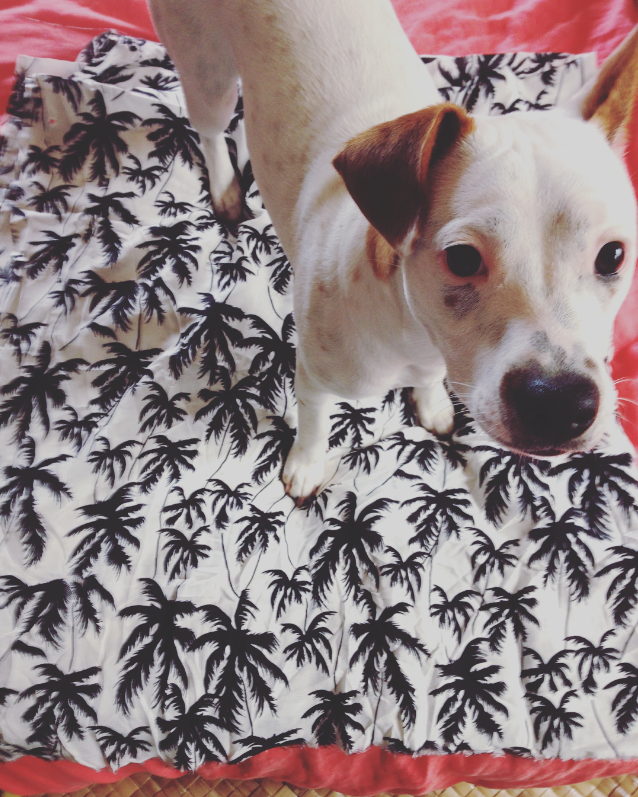
\includegraphics[width=0.3\textwidth,height=\textheight]{data/Paani.jpg}
\caption{\textbf{Figure 3. Pa'āni is \emph{beautiful} (and sassy).
Beware!}}
\end{figure}

Note in the coding above I used the html codes for centering the image
and the caption. You must leave a line between the first html call
\texttt{\textless{}center\textgreater{}}, the caption and image code,
and the end html code line of \texttt{\textless{}/center\textgreater{}}.

\hypertarget{figure-formatting}{%
\subsubsection{Figure formatting}\label{figure-formatting}}

\begin{itemize}
\item
  \texttt{fig.show=FALSE}: this will hide the figures you generate. This
  may be useful for some of those assumptions of ANOVA-- you want to see
  it, but do you want all of them in your final archived datafile? Maybe
  not.
\item
  \texttt{fig.width=5,\ fig.height=3}: The (graphical device) size of R
  plots in inches. This records your output figure as a graphical device
  using \emph{knitr} and will write this to files. There are other ways
  to edit figure size from this intial dimension (\emph{see below}). You
  can also specify the two (width and height using) \texttt{fig.dim}, as
  in the previous examle \texttt{fig.dim\ =\ c(5,\ 3)}
\item
  \texttt{out.width} and \texttt{out.height}: These set the output of a
  figure in output document. This is best to scale the image realtive to
  document dimensions, such as \texttt{out.width=\ "50\%"} would be 50\%
  of page width.
\item
  \texttt{fig.align}: gives you figure alignment as either: right,
  center, left.
\item
  \texttt{dev}: graphical devices, typically \texttt{png} (html) or
  \texttt{pdf} for LaTex.
\item
  \texttt{fig.cap}: caption your figure
\item
  \texttt{fig.show}: options here control your figures. Setting to
  \texttt{\textquotesingle{}asis\textquotesingle{}} will show plots in
  the location they were generated (similar to R terminal--this is the
  default). If you set to
  \texttt{\textquotesingle{}hide\textquotesingle{}} then the figures are
  generated but not shown in your output file. Another option below is
  my favorite.
\item
  \texttt{fig.show=\textquotesingle{}hold\textquotesingle{}}: this is a
  really cool option. This option holds you plots and doesn't display
  until the end of the code chunk. You can use it to place multiple
  figures side-by-side as long as the \texttt{out.width} is called. For
  example, two plots side-by-side at \texttt{out.widh="50\%"}
\end{itemize}

Now let's use some of these options to see how this code could be
executed.

\begin{Shaded}
\begin{Highlighting}[]
\CommentTok{\# use \textquotesingle{}data\textquotesingle{}, loaded above}

\FunctionTok{ggplot}\NormalTok{(data, }\FunctionTok{aes}\NormalTok{(}\AttributeTok{y=}\NormalTok{biomass, }\AttributeTok{x=}\NormalTok{Site, }\AttributeTok{fill=}\NormalTok{Status))}\SpecialCharTok{+}
  \FunctionTok{geom\_boxplot}\NormalTok{() }\SpecialCharTok{+}
  \FunctionTok{ylab}\NormalTok{(}\FunctionTok{expression}\NormalTok{(}\FunctionTok{paste}\NormalTok{(}\StringTok{"Biomass"}\NormalTok{, }\SpecialCharTok{\textasciitilde{}}\NormalTok{(mg}\SpecialCharTok{\textasciitilde{}}\NormalTok{cm}\SpecialCharTok{\^{}{-}}\DecValTok{2}\NormalTok{), }\AttributeTok{sep=}\StringTok{""}\NormalTok{)))}\SpecialCharTok{+}
  \FunctionTok{scale\_fill\_manual}\NormalTok{(}\AttributeTok{values=}\FunctionTok{c}\NormalTok{(}\StringTok{"lightblue"}\NormalTok{, }\StringTok{"mediumseagreen"}\NormalTok{))}\SpecialCharTok{+}
  \FunctionTok{theme\_classic}\NormalTok{()}

\FunctionTok{ggplot}\NormalTok{(data, }\FunctionTok{aes}\NormalTok{(}\AttributeTok{y=}\NormalTok{chla, }\AttributeTok{x=}\NormalTok{Site, }\AttributeTok{fill=}\NormalTok{Status))}\SpecialCharTok{+}
  \FunctionTok{geom\_boxplot}\NormalTok{() }\SpecialCharTok{+}
  \FunctionTok{ylab}\NormalTok{(}\FunctionTok{expression}\NormalTok{(}\FunctionTok{paste}\NormalTok{(}\StringTok{"Chlorophyll"}\NormalTok{, }\SpecialCharTok{\textasciitilde{}}\FunctionTok{italic}\NormalTok{(}\StringTok{"a"}\SpecialCharTok{+}\StringTok{"c"}\NormalTok{[}\DecValTok{2}\NormalTok{]), }\SpecialCharTok{\textasciitilde{}}\NormalTok{(mu}\SpecialCharTok{*}\NormalTok{g}\SpecialCharTok{\textasciitilde{}}\NormalTok{cm}\SpecialCharTok{\^{}{-}}\DecValTok{2}\NormalTok{), }\AttributeTok{sep=}\StringTok{""}\NormalTok{)))}\SpecialCharTok{+}
  \FunctionTok{scale\_fill\_manual}\NormalTok{(}\AttributeTok{values=}\FunctionTok{c}\NormalTok{(}\StringTok{"lightsalmon"}\NormalTok{, }\StringTok{"maroon"}\NormalTok{))}\SpecialCharTok{+}
  \FunctionTok{theme\_classic}\NormalTok{()}


\DocumentationTok{\#\#\#\# USING BASE R EXAMPLE}
\CommentTok{\#par(mar = c(4, 6, 0.2, 0.1))}
\CommentTok{\#plot(data$chla, pch=16, cex=1.2, col="coral",}
\CommentTok{\#      ylab=expression(paste("Chlorophyll", \textasciitilde{}italic("a"+"c"[2]), \textasciitilde{}(mu*g\textasciitilde{}cm\^{}{-}2), sep="")))}
\CommentTok{\#plot(data$biomass, pch=16, cex=1.2, col="mediumseagreen",}
\CommentTok{\#    ylab=expression(paste("Biomass", \textasciitilde{}(mg\textasciitilde{}cm\^{}{-}2), sep="")))}
\CommentTok{\#plot(data$chla, pch=16, cex=1.2, col="coral",}
\CommentTok{\#      ylab=expression(paste("Chlorophyll", \textasciitilde{}italic("a"+"c"[2]), \textasciitilde{}(mu*g\textasciitilde{}cm\^{}{-}2), sep="")))}
\end{Highlighting}
\end{Shaded}

\textbackslash begin\{figure\}

\{\centering \includegraphics[width=0.3\linewidth]{Intro-to-markdown_files/figure-latex/first plot example-1}
\includegraphics[width=0.3\linewidth]{Intro-to-markdown_files/figure-latex/first plot example-2}

\}

\textbackslash caption\{\textbf{Figure 4. Example of side-by-side plots
at 50\%, with a `fig hold' option}\}\label{fig:first plot example}
\textbackslash end\{figure\}

Let's try another plot and set the dimensions to 5'' wide and 3'' tall

\begin{Shaded}
\begin{Highlighting}[]
\FunctionTok{hist}\NormalTok{(data}\SpecialCharTok{$}\NormalTok{chla, }\AttributeTok{col=}\StringTok{"seagreen"}\NormalTok{, }\AttributeTok{freq=}\NormalTok{F, }\AttributeTok{main=}\StringTok{"Chlorophylls in coral symbionts"}\NormalTok{, }\AttributeTok{ylab=}\StringTok{"density"}\NormalTok{,}
      \AttributeTok{xlab=}\FunctionTok{expression}\NormalTok{(}\FunctionTok{paste}\NormalTok{(}\StringTok{"Chlorophyll"}\NormalTok{, }\SpecialCharTok{\textasciitilde{}}\FunctionTok{italic}\NormalTok{(}\StringTok{"a"}\SpecialCharTok{+}\StringTok{"c"}\NormalTok{[}\DecValTok{2}\NormalTok{]), }\SpecialCharTok{\textasciitilde{}}\NormalTok{(mu}\SpecialCharTok{*}\NormalTok{g}\SpecialCharTok{\textasciitilde{}}\NormalTok{cm}\SpecialCharTok{\^{}{-}}\DecValTok{2}\NormalTok{), }\AttributeTok{sep=}\StringTok{""}\NormalTok{)))}
\FunctionTok{par}\NormalTok{(}\AttributeTok{new=}\NormalTok{T)}
\FunctionTok{lines}\NormalTok{(}\FunctionTok{density}\NormalTok{(data}\SpecialCharTok{$}\NormalTok{chla),}\AttributeTok{lwd=}\DecValTok{3}\NormalTok{,}\AttributeTok{col=}\StringTok{"mediumseagreen"}\NormalTok{)}
\end{Highlighting}
\end{Shaded}

\begin{figure}

{\centering \includegraphics{Intro-to-markdown_files/figure-latex/test-plot-1} 

}

\caption{Figure 5. Chlorophyll *a* boxplot}\label{fig:test-plot}
\end{figure}

\emph{But something to consider\ldots{}}

R scripts in code chunks operate a bit differently than classic R
scripts. If you want to run your plot commands line-by-line you may need
to include calls, such as \texttt{with()} or \texttt{par(new=T)} to
specify that you do NOT want a new plot device to be made, but instead
to keep working on the device you have opened. So to execute the whole
chunk \texttt{hit\ the\ green\ arrow\ in\ the\ right\ of\ the\ chunk},
or highlight \emph{all} the lines you want to run and execute them this
way.

Let's run this code chunk but set an option for no figure caption.

\begin{Shaded}
\begin{Highlighting}[]
\CommentTok{\# use results="hide" here to suppress messages associate with "dev.off" and dev.print to save figure}

\NormalTok{MC.df}\OtherTok{\textless{}{-}}\NormalTok{data[(data}\SpecialCharTok{$}\NormalTok{Species}\SpecialCharTok{==}\StringTok{"MC"}\NormalTok{),] }\DocumentationTok{\#\# Montipora capitata alone}
\NormalTok{PC.df}\OtherTok{\textless{}{-}}\NormalTok{data[(data}\SpecialCharTok{$}\NormalTok{Species}\SpecialCharTok{==}\StringTok{"PC"}\NormalTok{),] }\DocumentationTok{\#\# Porites compress alone}

\FunctionTok{par}\NormalTok{(}\AttributeTok{mar =} \FunctionTok{c}\NormalTok{(}\DecValTok{4}\NormalTok{, }\DecValTok{4}\NormalTok{, }\DecValTok{3}\NormalTok{, }\FloatTok{0.1}\NormalTok{))}

\FunctionTok{plot}\NormalTok{(}\FunctionTok{density}\NormalTok{(MC.df}\SpecialCharTok{$}\NormalTok{biomass), }\AttributeTok{lwd=}\DecValTok{2}\NormalTok{, }\AttributeTok{col=}\StringTok{"darksalmon"}\NormalTok{, }\AttributeTok{xlim=}\FunctionTok{c}\NormalTok{(}\DecValTok{0}\NormalTok{,}\DecValTok{100}\NormalTok{), }\AttributeTok{main=}\StringTok{"Figure example. Tissue biomass in two coral species"}\NormalTok{, }\AttributeTok{cex.main=}\FloatTok{0.8}\NormalTok{, }\AttributeTok{xlab=}\FunctionTok{expression}\NormalTok{(}\FunctionTok{paste}\NormalTok{(}\StringTok{"Biomass"}\NormalTok{, }\SpecialCharTok{\textasciitilde{}}\NormalTok{(mg}\SpecialCharTok{\textasciitilde{}}\NormalTok{cm}\SpecialCharTok{\^{}{-}}\DecValTok{2}\NormalTok{), }\AttributeTok{sep=}\StringTok{""}\NormalTok{)))}
\FunctionTok{lines}\NormalTok{(}\FunctionTok{density}\NormalTok{(PC.df}\SpecialCharTok{$}\NormalTok{biomass), }\AttributeTok{lwd=}\DecValTok{2}\NormalTok{, }\AttributeTok{col=}\StringTok{"darkslategray3"}\NormalTok{, }\AttributeTok{yaxt=}\StringTok{"n"}\NormalTok{, }\AttributeTok{ylab=}\StringTok{""}\NormalTok{, }\AttributeTok{xaxt=}\StringTok{"n"}\NormalTok{, }\AttributeTok{xlab=}\StringTok{""}\NormalTok{)}
\FunctionTok{legend}\NormalTok{(}\StringTok{"topright"}\NormalTok{, }\AttributeTok{legend=}\FunctionTok{c}\NormalTok{(}\FunctionTok{expression}\NormalTok{(}\FunctionTok{italic}\NormalTok{(}\StringTok{"Montipora capitata"}\NormalTok{)), }\FunctionTok{expression}\NormalTok{(}\FunctionTok{italic}\NormalTok{(}\StringTok{"Porites compressa"}\NormalTok{))), }\AttributeTok{lwd=}\DecValTok{2}\NormalTok{, }\AttributeTok{col=}\FunctionTok{c}\NormalTok{(}\StringTok{"darksalmon"}\NormalTok{, }\StringTok{"darkslategray3"}\NormalTok{), }\AttributeTok{bty=}\StringTok{"n"}\NormalTok{)}
\end{Highlighting}
\end{Shaded}

\begin{figure}

{\centering \includegraphics{Intro-to-markdown_files/figure-latex/unnamed-chunk-3-1} 

}

\end{figure}

\begin{Shaded}
\begin{Highlighting}[]
\CommentTok{\# how to export the figure you made{-}{-}first print it, then save the device}
\CommentTok{\# many ways to do this, but this one works well in Markdown}
\CommentTok{\# notice you are specifying the folder (\textquotesingle{}figures\textquotesingle{}), which is where the figure will be exported to}

\FunctionTok{dev.print}\NormalTok{(pdf, }\StringTok{"figures/biomass in two species.pdf"}\NormalTok{, }\AttributeTok{height=}\DecValTok{4}\NormalTok{, }\AttributeTok{width=}\DecValTok{6}\NormalTok{) }\CommentTok{\# export in directory}
\FunctionTok{dev.off}\NormalTok{()}
\end{Highlighting}
\end{Shaded}

\hypertarget{now-lets-play}{%
\subsubsection{Now let's play!}\label{now-lets-play}}

In this chunk we will make use of some data of photopigments
(Chlorophyll \emph{a} concentrations cm\textsuperscript{-2}) in bleached
and pigmented corals. Some of the syntax here should be familiar\ldots{}

\begin{Shaded}
\begin{Highlighting}[]
\CommentTok{\# message = FALSE to hide any messages with exporting the figure with dev.off(), or anything else that R may generate. If you set warning=FALSE, warnings will be hidden as well. }

\FunctionTok{par}\NormalTok{(}\AttributeTok{mfrow=}\FunctionTok{c}\NormalTok{(}\DecValTok{1}\NormalTok{,}\DecValTok{1}\NormalTok{), }\AttributeTok{pty=}\StringTok{"sq"}\NormalTok{)}
\NormalTok{Status.label}\OtherTok{\textless{}{-}}\FunctionTok{c}\NormalTok{(}\StringTok{"Bleached"}\NormalTok{, }\StringTok{"Pigmented"}\NormalTok{) }\CommentTok{\# for x labels}

\CommentTok{\# sometimes loading the repo .csv gives an error message here, not sure why! Somehow the factor "Status" gets changed to integer incorrectly, should be fixed above in \textasciitilde{} line 190. In case, not, set it again.}

\NormalTok{data}\SpecialCharTok{$}\NormalTok{Status}\OtherTok{\textless{}{-}}\FunctionTok{as.factor}\NormalTok{(data}\SpecialCharTok{$}\NormalTok{Status)}

\FunctionTok{plot}\NormalTok{(chla}\SpecialCharTok{\textasciitilde{}}\NormalTok{Status, }\AttributeTok{data=}\NormalTok{data, }\AttributeTok{xaxt=}\StringTok{"n"}\NormalTok{, }\AttributeTok{col=}\StringTok{"salmon"}\NormalTok{,}
     \AttributeTok{ylab=}\FunctionTok{expression}\NormalTok{(}\FunctionTok{paste}\NormalTok{(}\StringTok{"Chlorophyll"}\NormalTok{, }\SpecialCharTok{\textasciitilde{}}\FunctionTok{italic}\NormalTok{(}\StringTok{"a"}\NormalTok{), }\SpecialCharTok{\textasciitilde{}}\NormalTok{(mu}\SpecialCharTok{*}\NormalTok{g}\SpecialCharTok{\textasciitilde{}}\NormalTok{cm}\SpecialCharTok{\^{}{-}}\DecValTok{2}\NormalTok{), }\AttributeTok{sep=}\StringTok{""}\NormalTok{)), }
     \AttributeTok{xlab=}\StringTok{"Coral Physiological State"}\NormalTok{, }
     \AttributeTok{main=}\StringTok{"Example Figure"}\NormalTok{)}
\FunctionTok{axis}\NormalTok{(}\DecValTok{1}\NormalTok{, }\AttributeTok{at=}\DecValTok{1}\SpecialCharTok{:}\DecValTok{2}\NormalTok{, }\AttributeTok{labels=}\NormalTok{Status.label) }\CommentTok{\# this plots new labels on the x axis (axis = 1)}
\end{Highlighting}
\end{Shaded}

\begin{figure}

{\centering \includegraphics{Intro-to-markdown_files/figure-latex/chlorophyll a figure-1} 

}

\caption{**Figure 5. Chlorophyll a density**. *Note: This caption was set in code chunk setting*}\label{fig:chlorophyll a figure}
\end{figure}

\begin{Shaded}
\begin{Highlighting}[]
\DocumentationTok{\#\#\#\#\# save the figure and export to directory? \#\#\#\#}
\CommentTok{\# in this case, there is a file in my directory names \textquotesingle{}figures\textquotesingle{} where I want plots to go}

\FunctionTok{dev.print}\NormalTok{(pdf, }\StringTok{"figures/Chlorophyll.figure.pdf"}\NormalTok{, }\AttributeTok{height=}\DecValTok{5}\NormalTok{, }\AttributeTok{width=}\DecValTok{5}\NormalTok{) }
\CommentTok{\# height and width set here for the output figure}
\FunctionTok{dev.off}\NormalTok{() }\CommentTok{\# close the object}
\end{Highlighting}
\end{Shaded}

I'm using
\texttt{dev.copy(pdf,\ "figures/Chlorophyll.figure.pdf",\ height=5,\ width=5)}
to print the devise, export it as a pdf, save in the folder names
``figures'', I'm naming the figure as ``Chlorophyll.figure.pdf'', and
exporting at 5x5 dimensions. Note the code chunk option is specifying to
print the figure in the Markdown at a smaller scale (4x4).

\hypertarget{examples}{%
\paragraph{Examples}\label{examples}}

\begin{itemize}
\tightlist
\item
  execute the code and see the returned results
\end{itemize}

\begin{Shaded}
\begin{Highlighting}[]
\NormalTok{chla}\OtherTok{\textless{}{-}}\NormalTok{(data}\SpecialCharTok{$}\NormalTok{chla)}
\FunctionTok{mean}\NormalTok{(chla)}
\end{Highlighting}
\end{Shaded}

\begin{verbatim}
## [1] 3.659065
\end{verbatim}

\begin{itemize}
\tightlist
\item
  see a code chunk in my markdown file, but it isn't executed if
  \texttt{eval=FALSE} is set
\end{itemize}

\begin{Shaded}
\begin{Highlighting}[]
\FunctionTok{mean}\NormalTok{(data}\SpecialCharTok{$}\NormalTok{chla)}
\end{Highlighting}
\end{Shaded}

\begin{itemize}
\tightlist
\item
  execute the code and hide results
  \texttt{results=\textquotesingle{}hide\textquotesingle{}}
\end{itemize}

\begin{Shaded}
\begin{Highlighting}[]
\NormalTok{chla}\OtherTok{\textless{}{-}}\NormalTok{(data}\SpecialCharTok{$}\NormalTok{chla)}
\FunctionTok{mean}\NormalTok{(chla)}
\end{Highlighting}
\end{Shaded}

\begin{itemize}
\tightlist
\item
  execute and show code and SEE the figure I generate, but hide results
  (returned data)\\
  \texttt{results=\textquotesingle{}hide\textquotesingle{},\ fig.height=4,\ fig.width=4,\ fig.align=\textquotesingle{}center\textquotesingle{}}
\end{itemize}

\begin{Shaded}
\begin{Highlighting}[]
\FunctionTok{par}\NormalTok{(}\AttributeTok{mfrow=}\FunctionTok{c}\NormalTok{(}\DecValTok{1}\NormalTok{,}\DecValTok{1}\NormalTok{))}
\FunctionTok{hist}\NormalTok{(chla, }\AttributeTok{col=}\StringTok{"gray85"}\NormalTok{, }\AttributeTok{xlab=}\FunctionTok{expression}\NormalTok{(}\FunctionTok{paste}\NormalTok{(}\StringTok{"Chlorophyll"}\NormalTok{, }\SpecialCharTok{\textasciitilde{}}\FunctionTok{italic}\NormalTok{(}\StringTok{"a"}\NormalTok{), }\SpecialCharTok{\textasciitilde{}}\NormalTok{(mu}\SpecialCharTok{*}\NormalTok{g}\SpecialCharTok{\textasciitilde{}}\NormalTok{cm}\SpecialCharTok{\^{}{-}}\DecValTok{2}\NormalTok{), }\AttributeTok{sep=}\StringTok{""}\NormalTok{)), }\AttributeTok{cex.main=}\FloatTok{0.8}\NormalTok{, }\AttributeTok{cex.axis=}\FloatTok{0.8}\NormalTok{, }\AttributeTok{cex.lab=}\FloatTok{0.8}\NormalTok{)}
\end{Highlighting}
\end{Shaded}

\begin{figure}

{\centering \includegraphics{Intro-to-markdown_files/figure-latex/unnamed-chunk-7-1} 

}

\caption{**Figure 6. Boxplot of chlorophyll *a* data**}\label{fig:unnamed-chunk-7}
\end{figure}

\begin{itemize}
\tightlist
\item
  make a two boxplots with ``bleached'' and ``non-bleached'' corals
  separated
\end{itemize}

\begin{Shaded}
\begin{Highlighting}[]
\FunctionTok{par}\NormalTok{(}\AttributeTok{mfrow=}\FunctionTok{c}\NormalTok{(}\DecValTok{1}\NormalTok{,}\DecValTok{2}\NormalTok{))}
\CommentTok{\# make figure 4 x 4 and center align}
\FunctionTok{hist}\NormalTok{(data}\SpecialCharTok{$}\NormalTok{chla[data}\SpecialCharTok{$}\NormalTok{Status}\SpecialCharTok{==}\StringTok{"B"}\NormalTok{], }\AttributeTok{col=}\StringTok{"darksalmon"}\NormalTok{, }\AttributeTok{xlab=}\FunctionTok{expression}\NormalTok{(}\FunctionTok{paste}\NormalTok{(}\StringTok{"Chlorophyll"}\NormalTok{, }\SpecialCharTok{\textasciitilde{}}\FunctionTok{italic}\NormalTok{(}\StringTok{"a"}\NormalTok{), }\SpecialCharTok{\textasciitilde{}}\NormalTok{(mu}\SpecialCharTok{*}\NormalTok{g}\SpecialCharTok{\textasciitilde{}}\NormalTok{cm}\SpecialCharTok{\^{}{-}}\DecValTok{2}\NormalTok{), }\AttributeTok{sep=}\StringTok{""}\NormalTok{)), }\AttributeTok{main=}\StringTok{"Bleached coral"}\NormalTok{, }\AttributeTok{cex.main=}\FloatTok{0.8}\NormalTok{, }\AttributeTok{cex.axis=}\FloatTok{0.8}\NormalTok{, }\AttributeTok{cex.lab=}\FloatTok{0.8}\NormalTok{)}
\FunctionTok{hist}\NormalTok{(data}\SpecialCharTok{$}\NormalTok{chla[data}\SpecialCharTok{$}\NormalTok{Status}\SpecialCharTok{==}\StringTok{"NB"}\NormalTok{], }\AttributeTok{col=}\StringTok{"darkslategray3"}\NormalTok{, }\AttributeTok{xlab=}\FunctionTok{expression}\NormalTok{(}\FunctionTok{paste}\NormalTok{(}\StringTok{"Chlorophyll"}\NormalTok{, }\SpecialCharTok{\textasciitilde{}}\FunctionTok{italic}\NormalTok{(}\StringTok{"a"}\NormalTok{), }\SpecialCharTok{\textasciitilde{}}\NormalTok{(mu}\SpecialCharTok{*}\NormalTok{g}\SpecialCharTok{\textasciitilde{}}\NormalTok{cm}\SpecialCharTok{\^{}{-}}\DecValTok{2}\NormalTok{), }\AttributeTok{sep=}\StringTok{""}\NormalTok{)), }\AttributeTok{main=}\StringTok{"Non{-}Bleached coral"}\NormalTok{, }\AttributeTok{cex.main=}\FloatTok{0.8}\NormalTok{, }\AttributeTok{cex.axis=}\FloatTok{0.8}\NormalTok{, }\AttributeTok{cex.lab=}\FloatTok{0.8}\NormalTok{)}
\end{Highlighting}
\end{Shaded}

\begin{figure}

{\centering \includegraphics{Intro-to-markdown_files/figure-latex/unnamed-chunk-8-1} 

}

\caption{**Figure 7. Boxplot of chlorophyll *a* data by physiological state**}\label{fig:unnamed-chunk-8}
\end{figure}

\ldots{} or just print the figure with \texttt{echo=FALSE} sans the code

\begin{figure}

{\centering \includegraphics{Intro-to-markdown_files/figure-latex/unnamed-chunk-9-1} 

}

\caption{**Figure 8. Separate boxplots of chlorophyll *a* among three reef sites**}\label{fig:unnamed-chunk-9}
\end{figure}

\ldots{} or show NOTHING with
\texttt{results=\textquotesingle{}hide\textquotesingle{},\ fig.show=FALSE}

\begin{Shaded}
\begin{Highlighting}[]
\FunctionTok{plot}\NormalTok{(chla}\SpecialCharTok{\textasciitilde{}}\NormalTok{Site, }\AttributeTok{data=}\NormalTok{data, }\AttributeTok{col=}\StringTok{"darkseagreen1"}\NormalTok{)}
\end{Highlighting}
\end{Shaded}

\hypertarget{make-a-table-of-summary-data}{%
\subsubsection{Make a table of summary
data}\label{make-a-table-of-summary-data}}

plot raw data `as is'

\begin{Shaded}
\begin{Highlighting}[]
\NormalTok{knitr}\SpecialCharTok{::}\FunctionTok{kable}\NormalTok{(data[}\FunctionTok{c}\NormalTok{(}\DecValTok{1}\SpecialCharTok{:}\DecValTok{5}\NormalTok{), }\FunctionTok{c}\NormalTok{(}\DecValTok{1}\SpecialCharTok{:}\DecValTok{10}\NormalTok{)], }\AttributeTok{digits =} \FunctionTok{c}\NormalTok{(}\DecValTok{0}\NormalTok{, }\DecValTok{0}\NormalTok{, }\DecValTok{0}\NormalTok{, }\DecValTok{0}\NormalTok{, }\DecValTok{0}\NormalTok{, }\DecValTok{0}\NormalTok{, }\DecValTok{0}\NormalTok{, }\DecValTok{3}\NormalTok{, }\DecValTok{3}\NormalTok{, }\DecValTok{3}\NormalTok{))}
\end{Highlighting}
\end{Shaded}

\begin{longtable}[]{@{}
  >{\raggedright\arraybackslash}p{(\columnwidth - 18\tabcolsep) * \real{0.1392}}
  >{\raggedright\arraybackslash}p{(\columnwidth - 18\tabcolsep) * \real{0.1266}}
  >{\raggedright\arraybackslash}p{(\columnwidth - 18\tabcolsep) * \real{0.0633}}
  >{\raggedright\arraybackslash}p{(\columnwidth - 18\tabcolsep) * \real{0.1013}}
  >{\raggedright\arraybackslash}p{(\columnwidth - 18\tabcolsep) * \real{0.0886}}
  >{\raggedright\arraybackslash}p{(\columnwidth - 18\tabcolsep) * \real{0.1266}}
  >{\raggedleft\arraybackslash}p{(\columnwidth - 18\tabcolsep) * \real{0.0633}}
  >{\raggedleft\arraybackslash}p{(\columnwidth - 18\tabcolsep) * \real{0.1139}}
  >{\raggedleft\arraybackslash}p{(\columnwidth - 18\tabcolsep) * \real{0.1013}}
  >{\raggedleft\arraybackslash}p{(\columnwidth - 18\tabcolsep) * \real{0.0759}}@{}}
\toprule\noalign{}
\begin{minipage}[b]{\linewidth}\raggedright
Time.point
\end{minipage} & \begin{minipage}[b]{\linewidth}\raggedright
Period
\end{minipage} & \begin{minipage}[b]{\linewidth}\raggedright
Site
\end{minipage} & \begin{minipage}[b]{\linewidth}\raggedright
Species
\end{minipage} & \begin{minipage}[b]{\linewidth}\raggedright
Status
\end{minipage} & \begin{minipage}[b]{\linewidth}\raggedright
Sample.ID
\end{minipage} & \begin{minipage}[b]{\linewidth}\raggedleft
Pair
\end{minipage} & \begin{minipage}[b]{\linewidth}\raggedleft
Depth.ft
\end{minipage} & \begin{minipage}[b]{\linewidth}\raggedleft
biomass
\end{minipage} & \begin{minipage}[b]{\linewidth}\raggedleft
chla
\end{minipage} \\
\midrule\noalign{}
\endhead
\bottomrule\noalign{}
\endlastfoot
2014 Oct & Bleaching & HIMB & MC & B & 3 & 2 & 0.667 & 21.223 & 2.572 \\
2014 Oct & Bleaching & HIMB & MC & NB & 4 & 2 & 0.667 & 27.318 &
4.766 \\
2014 Oct & Bleaching & HIMB & MC & B & 5 & 3 & 1.000 & 19.746 & 0.259 \\
2014 Oct & Bleaching & HIMB & MC & NB & 6 & 3 & 1.000 & 15.449 &
2.679 \\
2014 Oct & Bleaching & HIMB & PC & B & 9 & 5 & 1.667 & 26.273 & 0.043 \\
\end{longtable}

\begin{Shaded}
\begin{Highlighting}[]
\CommentTok{\# the digits call here is specifying the \# of decimals for each column}
\end{Highlighting}
\end{Shaded}

Or make summary data and include this table in your markdown

\begin{Shaded}
\begin{Highlighting}[]
\NormalTok{chl.mean}\OtherTok{\textless{}{-}}\FunctionTok{aggregate}\NormalTok{(chla}\SpecialCharTok{\textasciitilde{}}\NormalTok{Time.point }\SpecialCharTok{+}\NormalTok{ Site }\SpecialCharTok{+}\NormalTok{ Species }\SpecialCharTok{+}\NormalTok{ Status, data, mean)}
\NormalTok{biomass.mean}\OtherTok{\textless{}{-}}\FunctionTok{aggregate}\NormalTok{(biomass}\SpecialCharTok{\textasciitilde{}}\NormalTok{Time.point }\SpecialCharTok{+}\NormalTok{ Site }\SpecialCharTok{+}\NormalTok{ Species }\SpecialCharTok{+}\NormalTok{ Status, data, mean)}
\NormalTok{data.table}\OtherTok{\textless{}{-}}\FunctionTok{cbind}\NormalTok{(chl.mean[, }\FunctionTok{c}\NormalTok{(}\DecValTok{1}\SpecialCharTok{:}\DecValTok{5}\NormalTok{)], biomass.mean[,}\DecValTok{5}\NormalTok{])}
\FunctionTok{colnames}\NormalTok{(data.table)}\OtherTok{\textless{}{-}}\FunctionTok{c}\NormalTok{(}\StringTok{"Time Point"}\NormalTok{, }\StringTok{"Site"}\NormalTok{, }\StringTok{"Species"}\NormalTok{, }\StringTok{"Status"}\NormalTok{, }\StringTok{"mean chla"}\NormalTok{, }\StringTok{"mean AFDW"}\NormalTok{)}
\NormalTok{knitr}\SpecialCharTok{::}\FunctionTok{kable}\NormalTok{(data.table, }\AttributeTok{digits =} \FunctionTok{c}\NormalTok{(}\DecValTok{0}\NormalTok{,}\DecValTok{0}\NormalTok{,}\DecValTok{0}\NormalTok{,}\DecValTok{0}\NormalTok{, }\DecValTok{3}\NormalTok{, }\DecValTok{3}\NormalTok{))}
\end{Highlighting}
\end{Shaded}

\begin{longtable}[]{@{}llllrr@{}}
\toprule\noalign{}
Time Point & Site & Species & Status & mean chla & mean AFDW \\
\midrule\noalign{}
\endhead
\bottomrule\noalign{}
\endlastfoot
2014 Oct & HIMB & MC & B & 1.441 & 19.381 \\
2014 Oct & Reef 25 & MC & B & 1.177 & 16.729 \\
2014 Oct & Reef 44 & MC & B & 1.924 & 21.354 \\
2014 Oct & HIMB & PC & B & 0.681 & 30.966 \\
2014 Oct & Reef 25 & PC & B & 1.156 & 28.725 \\
2014 Oct & Reef 44 & PC & B & 0.837 & 38.478 \\
2014 Oct & HIMB & MC & NB & 5.187 & 27.214 \\
2014 Oct & Reef 25 & MC & NB & 3.673 & 26.553 \\
2014 Oct & Reef 44 & MC & NB & 4.543 & 28.493 \\
2014 Oct & HIMB & PC & NB & 10.336 & 37.186 \\
2014 Oct & Reef 25 & PC & NB & 6.350 & 47.681 \\
2014 Oct & Reef 44 & PC & NB & 7.341 & 42.946 \\
\end{longtable}

\begin{Shaded}
\begin{Highlighting}[]
\DocumentationTok{\#\#\#\#\#\#\#\#\#\#\#\#}
\CommentTok{\# other using methods for summary tables using \textquotesingle{}tidyverse\textquotesingle{} dplyr}
\NormalTok{data.table2}\OtherTok{\textless{}{-}}\NormalTok{ data }\SpecialCharTok{\%\textgreater{}\%}\NormalTok{ dplyr}\SpecialCharTok{::}\FunctionTok{select}\NormalTok{(Time.point, Site, Species, Status, chla, biomass) }\SpecialCharTok{\%\textgreater{}\%}
  \FunctionTok{group\_by}\NormalTok{(Time.point, Site, Species)}\SpecialCharTok{\%\textgreater{}\%}
  \FunctionTok{summarise}\NormalTok{(}\AttributeTok{mean.chla=}\FunctionTok{mean}\NormalTok{(chla), }\AttributeTok{mean.AFDW=} \FunctionTok{mean}\NormalTok{(biomass), }
            \AttributeTok{SE.chla=}\FunctionTok{std.error}\NormalTok{(chla), }\AttributeTok{SE.AFDW=}\FunctionTok{std.error}\NormalTok{(biomass))}

\CommentTok{\# knitr::kable(data.table2, digits = c(0,0,0, 3, 3, 3, 3), col.names = c("Time", "Site", "Species", "chla", "biomass", "SE{-}chla", "SE{-}biomass"))}
\end{Highlighting}
\end{Shaded}

\hypertarget{running-models}{%
\subsection{Running models}\label{running-models}}

Markdown makes running models easy. You can leave all candidate models
in the script or you can only report final models. In either case, it is
an easy way to keep your data from analysis easy to understand and to
QA/QC before publication

\hypertarget{lme-chlorophyll-model}{%
\subsubsection{LME chlorophyll model}\label{lme-chlorophyll-model}}

Load packages and look at structure of dataframe: notice I am hiding
these results with the \texttt{results=\ "hide"} option in the code
chunk

\begin{Shaded}
\begin{Highlighting}[]
\FunctionTok{str}\NormalTok{(data)}
\end{Highlighting}
\end{Shaded}

\hypertarget{fixed-and-random-effects}{%
\subsubsection{Fixed and random
effects}\label{fixed-and-random-effects}}

Run a linear mixed effect model, see the anova output, random effects,
and plot effects

\begin{Shaded}
\begin{Highlighting}[]
\NormalTok{mod}\OtherTok{\textless{}{-}}\FunctionTok{lmer}\NormalTok{(chla}\SpecialCharTok{\textasciitilde{}}\NormalTok{Species}\SpecialCharTok{+}\NormalTok{Site}\SpecialCharTok{*}\NormalTok{Status}\SpecialCharTok{+}\NormalTok{(}\DecValTok{1}\SpecialCharTok{|}\NormalTok{Pair), }\AttributeTok{data=}\NormalTok{data)}
\FunctionTok{anova}\NormalTok{(mod, }\AttributeTok{type=}\DecValTok{3}\NormalTok{) }\CommentTok{\# fixed effects}
\end{Highlighting}
\end{Shaded}

\begin{verbatim}
## Type III Analysis of Variance Table with Satterthwaite's method
##             Sum Sq Mean Sq NumDF DenDF F value    Pr(>F)    
## Species      30.28   30.28     1    52  7.4830  0.008499 ** 
## Site         17.69    8.84     2    52  2.1852  0.122678    
## Status      369.59  369.59     1    52 91.3201 4.868e-13 ***
## Site:Status  22.38   11.19     2    52  2.7652  0.072238 .  
## ---
## Signif. codes:  0 '***' 0.001 '**' 0.01 '*' 0.05 '.' 0.1 ' ' 1
\end{verbatim}

\begin{Shaded}
\begin{Highlighting}[]
\FunctionTok{ranova}\NormalTok{(mod) }\CommentTok{\# random effects}
\end{Highlighting}
\end{Shaded}

\begin{verbatim}
## ANOVA-like table for random-effects: Single term deletions
## 
## Model:
## chla ~ Species + Site + Status + (1 | Pair) + Site:Status
##            npar  logLik    AIC LRT Df Pr(>Chisq)
## <none>        9 -118.33 254.67                  
## (1 | Pair)    8 -118.33 252.67   0  1          1
\end{verbatim}

\begin{Shaded}
\begin{Highlighting}[]
\FunctionTok{plot}\NormalTok{(}\FunctionTok{allEffects}\NormalTok{(mod), }\AttributeTok{ylab=}\StringTok{"total chlorophyll/cm2"}\NormalTok{, }\AttributeTok{par.strip.text=}\FunctionTok{list}\NormalTok{(}\AttributeTok{cex=}\FloatTok{0.6}\NormalTok{))}
\end{Highlighting}
\end{Shaded}

\begin{figure}

{\centering \includegraphics{Intro-to-markdown_files/figure-latex/unnamed-chunk-13-1} 

}

\caption{**Figure 9. Model output fixed effect plots**}\label{fig:unnamed-chunk-13}
\end{figure}

\end{document}
